\section{输运问题}
\label{sec:transp-problem}

先看最简单的情形：一条直河以恒定速度$v$向右流动。用$u(x,t)$表示时刻$t$、位置$x$处水粒子携带的量，比如颜色的深浅。粒子不改变自己携带的值，时刻$t$位于$x$的粒子，在时刻$0$位于$x-vt$，所以
\begin{equation}
  u(x,t)=u_0(x-vt),
  \label{eq:transp-translate}
\end{equation}
其中$u_0$是初始分布。

设$u_0$可微，用链式法则计算式~\eqref{eq:transp-translate}的两个偏导数：
\[
  \partial_tu=-v\,u_0'(x-vt),\qquad \partial_xu=u_0'(x-vt).
\]
第一式加上第二式的$v$倍，右端抵消，得到恒定速度的\term{输运方程}（transport equation）
\begin{equation}
  \partial_tu+v\,\partial_xu=0.
  \label{eq:transp-constant}
\end{equation}

这个方程可以用两种视角读。站在岸上盯住固定位置，$\partial_tu$是看到的变化率：上游的值不断流过来，变化率等于$-v\,\partial_xu$。坐在随水漂流的小船上，周围的水相对自己不动，看到的值不变。式~\eqref{eq:transp-constant}说的就是这两种观察彼此一致。

图~\ref{fig:transp-shift}取$v=1$，初值是以$0$为中心、半宽为$1$的三角形。(a)中三个时刻的曲线形状相同，只是向右平移。(b)把同一个解画在$(x,t)$平面上，颜色的深浅沿斜线$x=x_0+t$保持不变，这些斜线就是粒子的轨迹。

\begin{BookInlineFigure}
  \centering
  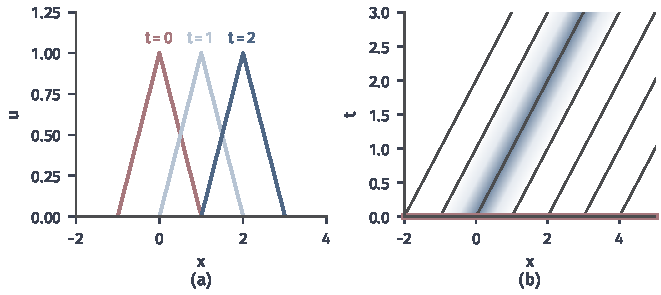
\includegraphics[width=112mm]{figures/06-differential-equations/02-partial-differential-equations/matplotlib/transp-shift/figure.pdf}
  \caption{恒定速度$v=1$的平移。(a)初值（红）和$t=1,2$时的解（蓝色由浅到深）。(b)解$u_0(x-t)$的时空热图，蓝色越深值越大，深灰斜线是粒子轨迹，红线是给定初值的$t=0$。}
  \label{fig:transp-shift}
\end{BookInlineFigure}

水流搬运墨水的比喻有它的边界。真实的墨水还会向四周扩散，边缘逐渐模糊；方程~\eqref{eq:transp-constant}中没有这一项，边缘再陡也不会变缓，初值的尖角和间断都被原样带走。扩散的效果由第~\ref{chap:diffusion-equations}章讨论。

\paragraph{一般的问题}
把水流换成随位置和时间变化的速度场$\bm{v}(\bm{x},t)$，同时允许粒子沿途获得或失去一些量，并考虑有边界的区域，就得到本章要研究的问题。

\begin{definition}[线性输运问题]
\label{def:transp-problem}
设$\Omega\subset\mathbb{R}^{d}$，$\bm{v}:\Omega\times[0,T]\to\mathbb{R}^{d}$是给定的速度场。\term{线性输运问题}（linear transport problem）是求$u(\bm{x},t)$，使
\begin{equation}
  \begin{cases}
    \partial_tu+\bm{v}\cdot\nabla u=f & \text{在}\ \Omega\times(0,T)\ \text{内},\\
    u(\cdot,0)=u_0 & \text{在}\ \Omega\ \text{上},\\
    u=g & \text{在入流边界}\ \Gamma_{-}(t)\ \text{上},
  \end{cases}
  \label{eq:transp-ibvp}
\end{equation}
其中$\bm{n}$是单位外法向，入流边界是
\begin{equation}
  \Gamma_{-}(t)=\{\bm{x}\in\partial\Omega:\bm{v}(\bm{x},t)\cdot\bm{n}(\bm{x})<0\}.
  \label{eq:transp-inflow-boundary}
\end{equation}
当$\Omega=\mathbb{R}^{d}$时，没有边界条件。
\end{definition}

方程中四个已知量的角色不同。
\begin{itemize}
  \item 速度场$\bm{v}$决定粒子往哪里走，它不携带任何场值。
  \item 初始场$u_0$给出时刻$0$在区域内的粒子所携带的值。
  \item 入流数据$g$给出后来从边界进入区域的粒子所携带的值。
  \item 源项$f$描述粒子沿途携带值的变化率，$f=1$表示每个粒子携带的值每单位时间增加$1$。
\end{itemize}

\paragraph{反向追踪}
某个时空点的值由哪些数据决定？从这一点出发，沿粒子的轨迹逆时间往回走，走到已知数据为止。下面以$\Omega=(0,1)$、$v=1/2$为例，此时入流边界只有左端点$x=0$。

如图~\ref{fig:transp-trace}(a)，从$P=(0.8,1)$往回走，轨迹是斜率固定的直线，时间退回$1$时，位置退回$0.5$，到达$(0.3,0)$，落在初始线上。从$Q=(0.2,1)$往回走，在退回时间$0.4$时已到达左端点$(0,0.6)$，落在入流边界上。没有源项时，这两点的值分别是
\[
  u(0.8,1)=u_0(0.3),\qquad u(0.2,1)=g(0.6).
\]

一般地，$(0,1)\times(0,T)$内的点$(x,t)$按下面的方式分成两类，由此得到解的表达式：
\begin{equation}
  u(x,t)=
  \begin{cases}
    u_0(x-vt), & x>vt,\\
    g(t-x/v), & x<vt.
  \end{cases}
  \label{eq:transp-inflow-solution}
\end{equation}
分界线$x=vt$是从角点$(0,0)$出发的轨迹。

\begin{BookInlineFigure}
  \centering
  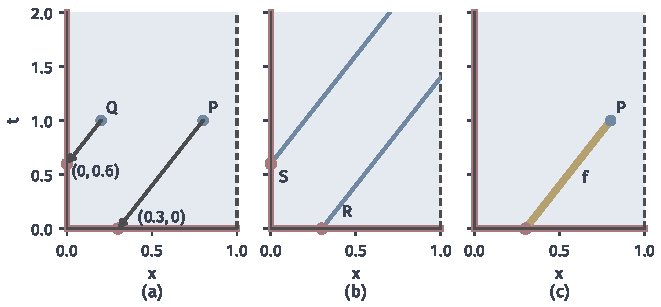
\includegraphics[width=112mm]{figures/06-differential-equations/02-partial-differential-equations/matplotlib/transp-trace/figure.pdf}
  \caption{区间$(0,1)$上$v=1/2$的追踪，红线是给数据的初始线和入流边界，深灰虚线是不给数据的出流边界。(a)从$P,Q$反向追踪到红线上的点。(b)从数据点$R,S$正向出发的影响范围（蓝线）。(c)有源项时，$P$的值还依赖黄色线段上的$f$。}
  \label{fig:transp-trace}
\end{BookInlineFigure}

\paragraph{正向追踪}
反过来，某个数据点影响哪些时空点？从数据点出发沿时间正向走即可。图~\ref{fig:transp-trace}(b)中，从$R$出发的影响范围只有一条线段，这条线段碰到右端点就离开了区域。这与第~\ref{chap:diffusion-equations}章的热方程很不一样，那里一点的扰动瞬间影响全局；与第~\ref{chap:wave-equations}章的波动方程也不同，那里一维的扰动沿左右两条线传播。

\paragraph{源项沿路径累积}
有源项时，粒子沿途不断获得新的量，$P$的值不只依赖轨迹的起点，还依赖整条轨迹上的$f$。如图~\ref{fig:transp-trace}(c)，黄色线段上每一处的$f$都对$u(P)$有贡献，而线段之外的$f$没有影响。这一累积的准确公式在第~\ref{sec:transp-characteristics}节给出。

\paragraph{入流数据与初值的衔接}
式~\eqref{eq:transp-inflow-solution}在分界线$x=vt$的两侧由不同的数据决定，解是否连续取决于角点上的相容性。图~\ref{fig:transp-inflow-solution}比较了两组数据。

(a)中$u_0=\tfrac12(1+\cos2\pi x)$，$g=\cos^{2}(\pi t/2)$。角点上$u_0(0)=g(0)=1$，解沿分界线连续。这里两侧的一阶导数也衔接，因为$u_0'(0)=g'(0)=0$。(b)中$u_0=0$，$g=1$，角点的值不一致，解在分界线上有一个高度为$1$的跳跃，并且这个跳跃沿分界线传播下去，不会被抹平。

\begin{BookInlineFigure}
  \centering
  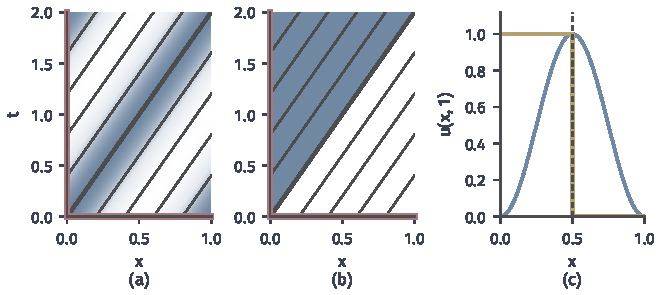
\includegraphics[width=112mm]{figures/06-differential-equations/02-partial-differential-equations/matplotlib/transp-inflow-solution/figure.pdf}
  \caption{$(0,1)$上$v=1/2$的解。(a)初值和入流相容，(b)初值$0$、入流$1$不相容。粗深灰线是分界线$x=t/2$，细深灰线是特征线，红线是给数据的边界，蓝色越深值越大。(c)$t=1$时的剖面，蓝线对应(a)，黄线对应(b)，虚线是分界线的位置。}
  \label{fig:transp-inflow-solution}
\end{BookInlineFigure}

右端点是出流边界，那里的值已由式~\eqref{eq:transp-inflow-solution}确定，不能再独立规定。图~\ref{fig:transp-inflow-solution}(b)的解在$x<t/2$处恒为$1$，在$x>t/2$处恒为$0$，它在分界线上不可导，方程不能逐点成立。这种解的含义留到第~\ref{sec:transp-weak}节讨论。
